\documentclass[12pt,a4paper]{report}

% Packages
\usepackage[utf8]{inputenc}
\usepackage{amsmath, amssymb}
\usepackage{graphicx}
\usepackage{hyperref}
\usepackage{geometry}
\usepackage{fancyhdr}
\usepackage{titlesec}
\usepackage{setspace}
\usepackage{listings}
\usepackage{color}
\usepackage{natbib}
\usepackage{tocbibind}
\usepackage{float}
\usepackage{dirtytalk}
\usepackage{dsfont}
\usepackage{algorithm}
\usepackage{algorithmic}

% Geometry settings
\geometry{
    a4paper,
    left=30mm,
    right=25mm,
    top=25mm,
    bottom=25mm,
}

% Header and Footer
\fancyhf{}
\fancyhead[L]{\leftmark}
\fancyhead[R]{\thepage}
\setlength{\headheight}{15pt}
\pagestyle{fancy}

% Title formatting
\titleformat{\chapter}[hang]{\LARGE\bfseries}{\thechapter.}{2pc}{}
\titleformat{\section}[hang]{\large\bfseries}{\thesection.}{1pc}{}

% Code Listings settings
\definecolor{codegray}{rgb}{0.5,0.5,0.5}
\definecolor{codegreen}{rgb}{0,0.6,0}
\definecolor{codeblue}{rgb}{0,0,0.9}
\definecolor{backcolour}{rgb}{0.95,0.95,0.92}

\lstdefinestyle{mystyle}{
    backgroundcolor=\color{backcolour},
    commentstyle=\color{codegreen},
    keywordstyle=\color{codeblue},
    numberstyle=\tiny\color{codegray},
    stringstyle=\color{codeblue},
    basicstyle=\ttfamily\footnotesize,
    breakatwhitespace=false,
    breaklines=true,
    captionpos=b,
    keepspaces=true,
    numbers=left,
    numbersep=5pt,
    showspaces=false,
    showstringspaces=false,
    showtabs=false,
    tabsize=2
}

\lstset{style=mystyle}

\newenvironment{acknowledgements}
  {\cleardoublepage\thispagestyle{plain}\chapter*{Acknowledgements}}
  {\cleardoublepage}

% Prevent duplicate destination identifiers
\hypersetup{pageanchor=true}

% Document start
\begin{document}

% Title Page
\begin{titlepage}
    \begin{center}
        \vspace*{1cm}

        \Huge
        \textbf{Incorporating Deep Descriptive Clustering into the DECCS Algorithm}

        \vspace{0.5cm}
        \LARGE
        for Enhanced Interpretability and Performance on AwA and APY Datasets

        \vspace{1.5cm}

        \textbf{Mehdi Benabed}

        \vfill

        A thesis submitted in partial fulfillment\\
        of the requirements for the degree of\\
        Master of Science in Computer Science

        \vspace{0.8cm}

        
\includegraphics[width=0.4\textwidth]{figs/Uni_Logo_2016.png}

        \Large
        Faculty of Computer Science\\
        University of Vienna\\
        Austria\\
        \today

    \end{center}
\end{titlepage}

% Abstract
\begin{abstract}
    \addcontentsline{toc}{chapter}{Abstract}
    This thesis introduces a novel approach to enhance the interpretability of the Deep Embedded Clustering with Consensus Representations (DECCS) algorithm by incorporating principles from the Deep Descriptive Clustering (DDC) framework. DECCS has shown significant advances in clustering precision but often falls short in terms of interpretability. This research aims to bridge this gap by refining the DECCS algorithm to not only generate clusters but also provide meaningful, cluster-level explanations that enhance transparency and comprehensibility in the clustering process.

The methodology involves adapting DECCS to effectively interface with specific datasets used in the DDC experimental framework, particularly the Animals with Attributes (AwA) and the aPascal \& aYahoo (aPY) datasets. This adaptation incorporates DDC’s symbolic level representations into DECCS, aiming to create a seamless integration between raw data clustering and semantic interpretability.

A significant aspect of this thesis is the integration of DDC’s interpretative capabilities with DECCS’s clustering method. This integration strives to maintain the high quality of cluster formation inherent to DECCS while elevating the level of interpretability. The dual focus ensures that the resulting predictions are both accurate and comprehensible, providing insights into the underlying structure and relationships within the data.

This thesis evaluates the integrated approach through extensive experiments, assessing both clustering performance and the quality of explanations generated. The evaluation includes comparisons with recent advancements and foundational algorithms in the field, demonstrating the efficacy of combining DECCS with DDC principles. By highlighting the advantages of this combination in practical clustering applications, the research contributes to the field of data clustering by offering a novel methodology that combines the efficiency of DECCS with the interpretative power of DDC.

Overall, this research sets a new benchmark for transparent, understandable, and insightful data analysis in various domains, addressing the increasing demand for interpretability and accountability in complex data clustering.
\end{abstract}

% Acknowledgements
%\begin{acknowledgements}
%    \addcontentsline{toc}{chapter}{Acknowledgements}
%    Write your acknowledgements here. Thank those who helped you with your research and thesis.
%\end{acknowledgements}

% Table of Contents
\tableofcontents
\listoffigures
\listoftables

% Chapters
\chapter{Introduction}
\section{Background}

The growing complexity of modern datasets necessitates a paradigm shift in algorithmic approaches, particularly in the realm of data clustering. While Deep Embedded Clustering with Consensus Representations (DECCS) has made significant strides in clustering precision, it highlights the critical limitation of interpretability within these advances. This limitation is becoming increasingly problematic in a landscape of data analysis that demands greater transparency and accountability \citep{Balachandran2009}. This research aims to address this gap by integrating the strengths of the Deep Descriptive Clustering (DDC) framework.

Interpretability in clustering is crucial for several reasons. In many real-world applications, such as healthcare, finance, and autonomous systems, the ability to understand and trust the decisions made by clustering algorithms can significantly impact decision-making processes. For instance, in healthcare, understanding why a group of patients has been clustered together can lead to better diagnoses and personalized treatments. Similarly, in finance, transparent clustering can help in risk assessment and fraud detection.

While DECCS excels in efficiently segmenting complex datasets, its opaque decision-making processes pose significant barriers in contexts where understanding the 'why' behind data clusters is as crucial as the 'what'. Integrating DDC principles can be considered a preliminary step towards interpreting the clustering process, thus enhancing utility and transparency in data analysis \citep{Saisubramanian2019}.

Furthermore, the practical implications of this integration are profound. By focusing on specific datasets, such as the Animals with Attributes (AwA) and the aPascal \& aYahoo (aPY), this research moves beyond theoretical advancements to demonstrate how the DECCS algorithm can be tailored to diverse datasets, thereby broadening its utility across various domains \citep{Ozyegen2022}.

The evolving nature of data clustering as an interdisciplinary field necessitates the convergence of accuracy and interpretability. By bridging the high precision of DECCS with the descriptive ability of DDC, this study contributes to a more holistic approach to data clustering \citep{Plant2011}.

In summary, this research is motivated by the need to reconcile the precision of computational clustering with the increasing demand for interpretability and transparency. By integrating DECCS with DDC principles, the study aims to set a new benchmark in data clustering that is both technically proficient and inherently comprehensible, thereby enhancing the utility and trustworthiness of clustering algorithms in diverse applications \citep{Tjoa2023}.

\section{Research Objectives}
The primary objectives of this research are as follows:
\begin{itemize}
    \item \textbf{Enhance Interpretability of DECCS}:
    \begin{itemize}
        \item \textbf{Objective}: Incorporate symbolic level representations from DDC into DECCS to generate meaningful, cluster-level explanations.
        \item \textbf{Research Question}: How can DDC be integrated into DECCS to improve the interpretability of clustering results?
    \end{itemize}
    \item \textbf{Maintain or Improve Clustering Performance}:
    \begin{itemize}
        \item \textbf{Objective}: Ensure that the integration of DDC does not compromise the clustering performance of DECCS and ideally enhances it.
        \item \textbf{Research Question}: What impact does the integration of DDC have on the clustering performance of DECCS?
    \end{itemize}
    \item \textbf{Evaluate on AwA and aPY Datasets}:
    \begin{itemize}
        \item \textbf{Objective}: Test the integrated DECCS-DDC approach on the AwA and aPY datasets to validate the improvements in interpretability and performance.
        \item \textbf{Research Question}: How does the integrated approach perform on the AwA and aPY datasets compared to the standalone DECCS and DDC methods?
    \end{itemize}
\end{itemize}

\chapter{Literature Review}
\section{Deep Embedded Clustering with Consensus Representations (DECCS)}

The DECCS paper \citep{Miklautz2021}, "Deep Clustering With Consensus Representations," presents an innovative approach in the field of deep clustering. It addresses the limitations of existing deep clustering methods that are typically designed for a single clustering model, like k-means, spectral clustering, or Gaussian mixture models. These methods often fall short when their underlying assumptions are not met by the data.

DECCS (Deep Embedded Clustering with Consensus Representations) proposes a novel method that combines deep learning and clustering to improve both the learned representation and the performance of multiple heterogeneous clustering algorithms simultaneously. This approach is a significant departure from current deep clustering (DC) and consensus clustering (CC) methods, which typically focus on single models and may not effectively handle high-dimensional datasets or non-linear transformations.

\subsection{Related Work in Consensus Clustering and Deep Clustering}

\begin{itemize}
\item \textbf{Consensus Clustering (CC):} Traditional CC methods create robust clustering by combining multiple solutions into a single partition. However, they often don't access the original data features and are limited to linear transformations or specific clustering types like k-means. DECCS overcomes these limitations by learning a non-linear consensus function for the representation as follows:

\begin{itemize}
    \item \(\Theta\) - Set of learnable parameters of the encoder.
    \item \textit{enc} - Encoder function that maps data points to a lower-dimensional embedded space.
    \item \(X\) - An \(N \times D\) dimensional input data matrix.
    \item \(Z\) - An \(N \times d\) dimensional embedded data matrix, where \(Z = \textit{enc}(X)\) and \(d < D\).
    \item \(\mathcal{E}\) - Set of heterogeneous clustering algorithms.
    \item \(k_i\) - Number of clusters for the \(i^{th}\) clustering algorithm \(e_i\).
    \item \(\pi_i\) - Clustering result for the \(i^{th}\) clustering algorithm, where \(\pi_i = e_i(Z)\).
    \item \(Z_{cr}\) - Consensus representation that maximizes the objective function involving normalized mutual information across clustering results.
    \item \(c\) - Normalization constant for the objective function, defined as \(c = \frac{2}{|\mathcal{E}|^2-|\mathcal{E}|}\) to ensure the equation sums to one.
    \item \(f_{\Theta}\) - Objective function for consensus representation.
    \item \(NMI\) - Normalized Mutual Information, used as a measure in the objective function.
\end{itemize}

\(Z_{cr}\) maximizes the following objective function:

\[
f_{\Theta} = c \sum_{i=1}^{|\mathcal{E}|} \sum_{j>i}^{|\mathcal{E}|} NMI(e_i(\textit{enc}(\Theta)(X)), e_j(\textit{enc}(\Theta)(X))),
\]
where
\[
Z_{cr} := \textit{enc}_{\Theta_{cr}}(X),
\]
and \(\textit{enc}_{\Theta_{cr}}\) is the \textit{consensus representation function} and \(c\) is a normalization constant
\[
c = \frac{2}{|\mathcal{E}|^2-|\mathcal{E}|}
\]
for the equation to sum to one.

\item \textbf{Deep Clustering (DC):} Existing DC methods are typically tailored to a single clustering model, which may not always align with the data's characteristics. Methods like SpectralNet, DEC, and VaDE focus on specific clustering algorithms but do not account for the diversity of data types and clustering requirements found in complex datasets. For instance, DEC \citep{Xie2016} introduces a novel approach to clustering by combining representation learning with clustering in a deep learning framework. DEC uses a deep neural network to learn a mapping from the data space to a lower-dimensional feature space, where clustering is performed. The DEC algorithm iteratively refines cluster centers using a clustering loss function, significantly improving clustering results on various datasets. However, DEC struggles with handling different types of data and may not provide satisfactory results for highly heterogeneous datasets.

\item \textbf{Variational Autoencoders (VAE):} Introduced by Kingma and Welling (2014) \citep{Kingma2014}, VAE is a powerful generative model that learns a probabilistic mapping from data to a latent space and back. VAEs combine principles from variational inference and deep learning, making them effective for learning complex data distributions and generating new data samples. The VAE framework consists of an encoder that maps input data to a latent space and a decoder that reconstructs the data from the latent space. VAEs are particularly useful in clustering because they create smooth and continuous latent spaces where similar data points remain close in the latent space, thus facilitating improved clustering performance. However, VAEs also face limitations in dealing with the variability and complexity of real-world data.
\end{itemize}

\subsection{Methodology of DECCS}

DECCS is innovative in using a consensus representation learning approach, where it employs an autoencoder (AE) to learn a simplified representation of data. This simplification reduces ambiguity and increases the similarity of clustering results across different ensemble members, thus improving the overall clustering performance. The method involves three main steps: generating base partitions, approximating each partition with a classifier, and then updating the consensus representation.

\begin{figure}
\centering
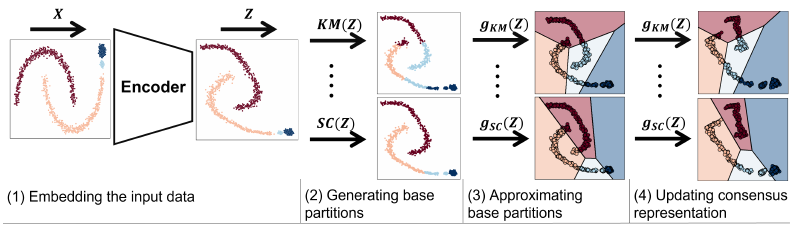
\includegraphics[width=1\textwidth]{figs/deccs.png}
    \caption{Visualisation of one round of DECCS\citep{Miklautz2021}. (1) The encoder is used to embed data points $X$. (2) Clustering results are generated by applying ensemble members $\mathcal{E} = \{KM, \ldots, SC\}$ to $Z$. (3) Classifiers $g_i$ are trained to predict the corresponding cluster labels $\pi_i$ from $Z$. (4) $Z$ is updated via minimizing $\mathcal{L}$.}
\label{fig:pipeline}
\end{figure}

\subsection{Experimental Evaluation}

DECCS was evaluated across various datasets, including MNIST, Fashion-MNIST, Kuzushiji-MNIST, USPS, and others. The experimental setup involved using a feed-forward AE architecture and setting specific hyperparameters for DECCS, like the consensus weight (cons) and sampling size (n). The evaluation metrics included normalized mutual information (NMI) and adjusted rand index (ARI), focusing on the agreement within an ensemble and cluster performance. DECCS showed improved agreement and cluster performance across all ensemble members, outperforming several relevant baselines from deep clustering and consensus clustering.

In summary, DECCS represents a significant advancement in deep clustering, effectively addressing the challenges of integrating multiple clustering methods. Its ability to learn a consensus representation that maximizes ensemble agreement marks a key innovation in this field.

\section{Deep Descriptive Clustering (DDC)}

The paper "Deep Descriptive Clustering" \citep{Zhang2021} by Hongjing Zhang and Ian Davidson explores a novel approach to clustering complex data such as images, text, and graphs, with a focus on explainable AI (XAI). This approach is particularly significant in the context of unsupervised learning like clustering, where explanations are crucial at the model level rather than just the instance level. The paper introduces the Deep Descriptive Clustering (DDC) framework, which combines deep clustering with cluster-level explanations. This framework is unique in its ability to learn from both sub-symbolic (clustering) and symbolic (explanation) levels simultaneously.

\subsection{Key Aspects of Deep Descriptive Clustering (DDC)}

\textbf{Clustering Objective:} DDC maximizes the mutual information between the empirical distribution on the inputs and the induced clustering labels. This approach is inspired by the discriminative clustering model, which has fewer assumptions about the data.

\textbf{Class-Level Explanation Objective:} DDC uses Integer Linear Programming (ILP) to generate concise and orthogonal explanations for each cluster. This method addresses the limitations of existing approaches that either require interpretable features or are post-hoc explanations that don't inform the clustering process.

\textbf{Self-Generated Pairwise Loss Term:} This innovative component reconciles inconsistencies between clustering and explanation by introducing self-generated constraints. The method leverages semantic tags to generate explanations and reshape clustering features, improving the overall clustering quality.

\begin{figure}
\centering
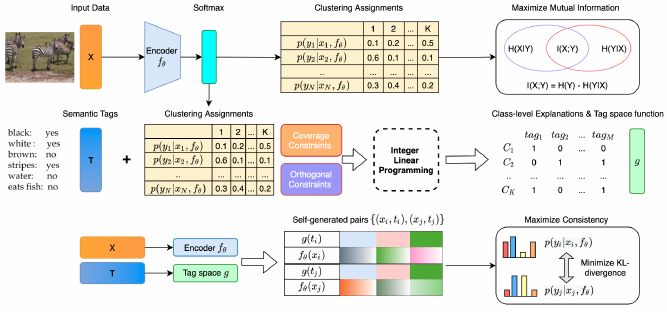
\includegraphics[width=1\textwidth]{figs/dec.png}
    \caption{The framework of deep descriptive clustering (DDC). DDC consists of one clustering objective, one sub-symbolic explanation objective, and one self-generated objective to maximize the consistency between clustering and explanation modules.}
\label{fig:ddc}
\end{figure}

\subsection{Experiments and Findings}

The paper evaluates the DDC framework on datasets like Attribute Pascal and Yahoo (aPY) and Animals with Attributes (AwA), comparing it against other methods in terms of explanation quality and clustering performance. DDC outperforms competitive baselines in clustering performance and offers high-quality cluster-level explanations. The evaluation metrics used include Tag Coverage (TC) and Inverse Tag Frequency (ITF), along with Normalized Mutual Information (NMI) and Clustering Accuracy (ACC) for a comprehensive assessment.

\subsection{Conclusion and Future Directions}

The paper concludes that the deep descriptive clustering model successfully clusters and generates high-quality cluster-level explanations. It emphasizes the model's potential in dealing with noisy semantic features and exploring novel forms of explanations beyond ontologies. Future work is directed towards enhancing the explainability of clustering models in diverse data contexts. In summary, this paper presents a groundbreaking approach in the field of explainable AI, offering a robust framework for both clustering and generating meaningful explanations.

\section{Related Works}

\subsection{Deep Embedded Clustering: A General Approach to Clustering Arbitrary Similarity Measures by J. Xie, R. Girshick, and A. Farhadi (2016)}

Deep Embedded Clustering (DEC) is a seminal work by Xie, Girshick, and Farhadi (2016) that introduces a novel approach to clustering by combining representation learning with clustering in a deep learning framework. DEC uses a deep neural network to learn a mapping from the data space to a lower-dimensional feature space, where clustering is performed. The key innovation of DEC is its use of an unsupervised learning algorithm that iteratively refines the cluster centers and improves clustering quality through a clustering loss function.

The DEC algorithm involves two main steps: the initial embedding of data into a lower-dimensional space using a stacked autoencoder, and the subsequent clustering of these embeddings using a clustering objective that minimizes the Kullback-Leibler (KL) divergence between the soft assignments and a target distribution. This iterative process allows the algorithm to refine both the embeddings and the cluster centers, resulting in better clustering performance.

DEC has been shown to significantly improve clustering results on various datasets compared to traditional methods, establishing its effectiveness and robustness. This work is foundational in demonstrating the power of deep learning for clustering tasks, and it has inspired numerous subsequent studies in the field of deep clustering \citep{Xie2016}.

\begin{figure}[h]
    \centering
    %\includegraphics[width=0.8\textwidth]{dec_architecture.png}
    \caption{Architecture of the Deep Embedded Clustering (DEC) model. The model consists of a stacked autoencoder followed by a clustering layer. The autoencoder learns a low-dimensional representation of the data, which is then clustered using a clustering objective.}
    \label{fig:dec_architecture}
\end{figure}

\subsection{Auto-Encoding Variational Bayes by D. P. Kingma and M. Welling (2014)}

Auto-Encoding Variational Bayes (VAE) is a powerful generative model introduced by Kingma and Welling (2014) that learns a probabilistic mapping from data to a latent space and back. VAEs combine principles from variational inference and deep learning, making them highly effective for learning complex data distributions and generating new data samples.

The VAE framework consists of two main components: an encoder that maps the input data to a latent space, and a decoder that reconstructs the data from the latent space. The encoder produces parameters for a probability distribution in the latent space, typically Gaussian, from which latent variables are sampled. The decoder then reconstructs the input data from these latent variables. The training objective of a VAE includes a reconstruction loss, which ensures the reconstructed data is similar to the original data, and a regularization term, which ensures the latent space distribution is close to a prior distribution, typically Gaussian.

VAEs are particularly useful in clustering because they create smooth and continuous latent spaces where data points that are similar in the original space remain close in the latent space. This property makes it easier to apply clustering algorithms to the latent representations learned by the VAE, leading to improved clustering performance \citep{Kingma2014}.

\begin{figure}[h]
    \centering
%    \includegraphics[width=0.8\textwidth]{vae_architecture.png}
    \caption{Architecture of the Variational Autoencoder (VAE) model. The encoder maps input data to a latent space, and the decoder reconstructs the data from the latent space. The model is trained to minimize reconstruction loss and regularization loss.}
    \label{fig:vae_architecture}
\end{figure}

\subsection{Explainable-by-Design Algorithms}

Explainable-by-design algorithms, as conceptualized by researchers like Bertsimas et al. (2020) and Moshkovitz et al. (2020), represent a class of methods that inherently integrate interpretability into the clustering process. These algorithms are designed with a dual purpose: to perform clustering tasks and simultaneously provide understandable explanations for the clustering outcomes. By utilizing interpretable features, such as simple and easily understandable attributes, these methods ensure that both the process and results of clustering are transparent and comprehensible to users.

The fundamental approach of these algorithms is to employ interpretable features in the construction of decision trees or other similar models, which then serve as the basis for both clustering and explaining the grouped data. For instance, in a clustering task involving customer segmentation, an explainable-by-design algorithm might use customer attributes like age, location, or purchasing habits, which are inherently interpretable, to form clusters and provide explanations for why certain customers are grouped together.

However, the application of these algorithms has certain limitations, particularly when dealing with complex data types such as images or graphs. In such scenarios, the raw features (like pixel values in images or edge connections in graphs) are often high-dimensional, less interpretable, and do not lend themselves to straightforward explanations. This limitation restricts the effectiveness of explainable-by-design algorithms in scenarios where the data complexity exceeds the interpretability of the features used for clustering.

\subsection{Post-processing Explanation Methods}

Post-processing explanation methods, developed by researchers like Davidson et al. (2018) and Sambaturu et al. (2020) \citep{Sambaturu2020}, take a different approach to explainability in clustering. Unlike explainable-by-design algorithms, these methods do not integrate explainability into the clustering process itself. Instead, they focus on generating explanations for pre-existing clustering results. These methods typically employ an additional set of features, often referred to as semantic tags, which are used to post-process and explain the outcomes of the clustering algorithms.

For example, in a clustering task involving document classification, a post-processing method might use semantic tags related to the content or theme of the documents to provide explanations for why certain documents are grouped together. This approach is algorithm-agnostic, meaning it can be applied to the results of any clustering algorithm, regardless of how the initial clustering was performed.

However, a critical limitation of post-processing explanation methods is that they may not fully leverage the information available from the additional features. Since these methods are applied after the clustering has been completed, they often rely on the inherent quality of the initial clustering. If the original clustering does not align well with the semantic tags used for explanation, the resulting explanations can be suboptimal or less meaningful. This disconnect between the clustering process and the post-hoc explanation phase can lead to explanations that do not fully capture the nuances or the rationale behind the formed clusters.

\subsection{Other Related Works}

Other significant contributions to the field of interpretable clustering include the works by Rishinanda and Sebag (2021) on deep discriminative clustering analysis, Liu et al. (2022) on generating natural language descriptions for clusters, and Chhajer and Moniri (2022) on using disentangled representations for clustering. These studies have advanced the understanding of how deep learning techniques can be leveraged to improve both the performance and interpretability of clustering algorithms.

Rishinanda and Sebag (2021) propose a deep learning approach that combines representation learning and discriminative clustering, aiming to produce well-separated and interpretable clusters. Liu et al. (2022) introduce a framework for generating natural language descriptions for clusters, enhancing the accessibility of clustering results to non-experts. Chhajer and Moniri (2022) focus on disentangled representations, which separate different explanatory factors in the data, making the clustering results more understandable.

These advancements demonstrate the ongoing efforts to make clustering algorithms not only more accurate but also more interpretable, bridging the gap between complex data analysis and human understanding \cite{Rishinanda2021, Liu2022, Chhajer2022}.

\chapter{Methodology}
To develop a system that combines Deep Embedded Clustering with Consensus Representations (DECCS) and Deep Descriptive Clustering (DDC), this methodology leverages the strengths of both methods to create an efficient and interpretable clustering system. This approach ensures that the resulting clusters are not only robust but also provide meaningful insights.

\subsubsection{Initial Clustering with DECCS}
\begin{itemize}
\item \textbf{Selection of Clustering Algorithms}: The process begins with the careful selection of a diverse array of clustering algorithms. Each algorithm should offer unique strengths and perspectives, ensuring that the DECCS ensemble encompasses a wide range of clustering approaches. This diversity is key to capturing the multifaceted nature of complex datasets.

\item \textbf{Application of DECCS Methodology}: DECCS synthesizes the varied clustering results into a unified consensus representation. This step involves processing the dataset through each selected algorithm and then using DECCS to find common ground among the disparate clustering outcomes. The aim is to achieve a consensus that balances the insights from each algorithm, resulting in robust and comprehensive clustering.
\end{itemize}


\subsubsection{Generating Explanations with DDC}
\begin{itemize}
\item \textbf{Mapping Features to Tags}: For the clusters formed through DECCS, the next step involves mapping complex data features onto a set of interpretable tags or labels. This process transforms high-dimensional, abstract data features into a more easily understood format, facilitating the generation of meaningful cluster explanations.

\item \textbf{Solving the ILP Problem}: Utilizing DDC’s Integer Linear Programming (ILP) methodology, concise and meaningful explanations for each cluster are generated. This step leverages the mapped tags to create explanations that not only describe the clusters but also offer insights into their underlying structure and relationships.
\end{itemize}

%\begin{algorithm}[H]
%\caption{Generating Explanations with DDC}
%\begin{algorithmic}[1]
%\State
%\textbf{Input:} Clusters from DECCS, feature-tag mapping
%\For{each cluster $c$}
%    \State Map features of $c$ to tags
%    \State Solve ILP to find the most representative tags for $c$
%    \State Generate explanation for $c$ using selected tags
%\EndFor
%\State \textbf{Output:} Explanations for all clusters
%\end{algorithmic}
%\end{algorithm}


\subsubsection{Integration of Pairwise Loss Function}
\begin{itemize}
\item \textbf{Modification of DECCS Framework}: The DECCS training algorithm is enhanced by integrating DDC's pairwise loss function. This additional loss component addresses discrepancies between the clustering feature space and the tag-based explanation space, thereby aligning the clustering process more closely with the generated explanations.

\item \textbf{Implementation of Pairwise Loss}: During training, instances within each mini-batch that are close in the tag space but far apart in the clustering feature space are identified. The pairwise loss is then calculated based on these discrepancies and used to update the model parameters during backpropagation.
\end{itemize}

\begin{equation}
\mathcal{L}_{pairwise} = \sum_{i,j} \mathds{1}_{[d_{tag}(i,j) < \epsilon]} \cdot \left( d_{feature}(i,j) \right)^2
\end{equation}

\subsubsection{Balancing Loss Components}
\textbf{Harmonization of Loss Functions}: Balancing the new pairwise loss with the existing loss functions in DECCS is essential. This balancing act often requires careful hyperparameter tuning to ensure that neither the clustering objective nor the explanation objective dominates, thus maintaining a harmonious integration of the two.

\subsubsection{Iterative Optimization and Refinement}
\begin{itemize}
\item \textbf{Iterative Process Establishment}: An iterative loop is established where both clustering (via DECCS) and explanations (via DDC) are refined in tandem. After updating the DECCS clustering with the latest data representation, DDC is applied to generate explanations for the new clusters.

\item \textbf{Feedback Loop Creation}: The explanations generated by DDC inform subsequent iterations of clustering in DECCS. Insights from the explanations are used to adjust the representation learning in DECCS or to fine-tune the consensus mechanism.

\item \textbf{Consistency Monitoring}: Consistency between clustering outputs and their explanations is continuously monitored. This step ensures that the explanations accurately reflect the clusters, and adjustments are made as necessary to both the clustering mechanism and the explanation generation process.

\item \textbf{Convergence Criteria Definition}: Criteria for convergence in this iterative optimization process are established. These could be based on the stability of cluster assignments over iterations, improvement in explanation quality, or a set number of iterations.

\item \textbf{Evaluation and Refinement Post Iteration}: Each iteration ends with an evaluation of both clustering and explanation quality. The models are then refined based on these evaluations to enhance clustering performance and the relevance and quality of explanations.
\end{itemize}


\subsubsection{Finalization of the Model}
\textbf{Model Finalization}: Upon achieving alignment between well-defined clusters and their corresponding explanations, the iterative process concludes. The final model is a synthesis of DECCS’s effective clustering capabilities and DDC’s interpretative explanations.

\subsubsection{Performance and Interpretability Evaluation}
\begin{itemize}
\item \textbf{Evaluation Metrics}: The performance of the integrated DECCS-DDC approach will be evaluated using clustering metrics such as Normalized Mutual Information (NMI) and Adjusted Rand Index (ARI). Interpretability will be assessed using metrics such as Tag Coverage (TC) and Inverse Tag Frequency (ITF).

\item \textbf{Experimental Setup}: The integrated approach will be tested on the Animals with Attributes (AwA) and aPascal \& aYahoo (aPY) datasets. The evaluation will compare the performance and interpretability of the integrated DECCS-DDC approach against the standalone DECCS and DDC methods.
\end{itemize}



\chapter{Results}
\input{chapters/results}

\chapter{Discussion}
The integration of Deep Descriptive Clustering (DDC) into the Deep Embedded Clustering with Consensus Representations (DECCS) framework represents an innovative application of data clustering. This research should demonstrate that the fusion of these two methodologies can effectively address the dual challenge of achieving high-precision clustering while enhancing interpretability and transparency in complex datasets like Animals with Attributes (AwA) and aPascal \& aYahoo (aPY).

One of the key strengths of this integrated approach is its ability to leverage the interpretative capabilities of DDC to inform and refine the clustering process in DECCS. By incorporating explanations that are both concise and meaningful, this methodology provides valuable insights into the structure and relationships within the data, which were mostly obscured in standard clustering approaches. This aspect is especially crucial in dealing with complex and high-dimensional datasets, where traditional clustering techniques often struggle to provide clear insights.

The iterative process of alternating between clustering updates (using DECCS) and generating explanations (using DDC) should ensure that both components inform and enhance each other. This synergy should not only improve the clustering performance but also the relevance and quality of the explanations generated, thus making the clustering results more understandable and actionable.

The combination of DECCS and DDC into a unified methodology marks a notable innovation in the field of data clustering. This approach should not only maintain the high quality of cluster formation inherent in DECCS but also should also elevate the level of interpretability through DDC’s explanatory framework. The successful application of this integrated method to the AwA and aPY datasets should serve as a testament to its efficacy and potential applicability in various other domains.

Furthermore, this research should contribute to the broader objective of making machine learning models, particularly in unsupervised learning scenarios like clustering, more transparent and interpretable. The ability to generate understandable and meaningful explanations for clustering decisions is a significant step forward in the field of explainable AI.

In summary, this study should set a new benchmark in data clustering, offering a methodology that is not only technically proficient but also inherently comprehensible. It should pave the way for future research in developing more transparent, understandable, and insightful data analysis techniques, thereby enhancing the utility and trustworthiness of clustering algorithms in a wide range of applications.

\chapter{Conclusion}
\input{chapters/conclusion}

% Appendices
\appendix
\chapter{Appendix A}
\input{appendices/appendix_a}

\chapter{Appendix B}
\input{appendices/appendix_b}

\bibliographystyle{plainnat}
\bibliography{bibliography}

\end{document}
